\documentclass[conference]{IEEEtran}
\IEEEoverridecommandlockouts
% The preceding line is only needed to identify funding in the first footnote. If that is unneeded, please comment it out.
\usepackage{cite}
\usepackage{amsmath,amssymb,amsfonts}
\usepackage{algorithm2e}
\usepackage{graphicx}
\usepackage{textcomp}
\usepackage{xcolor}
\usepackage{multirow}
\usepackage{subfigure}
\usepackage{comment}
\usepackage{url}
\def\BibTeX{{\rm B\kern-.05em{\sc i\kern-.025em b}\kern-.08em
    T\kern-.1667em\lower.7ex\hbox{E}\kern-.125emX}}
\newcommand{\virgolette}[1]{``#1''}    
\newcommand{\attenzione}[1]{\textcolor{magenta}{#1}}
\newcommand{\omitted}[1]{\emph{omitted for blind review}}


\begin{document}

%costo, tracceconsole log
%an algorithm for PV optimal placement and configuration
%Configuration and optimal placement of PV systems
%OCCP: Optimal Configuration and Placement of PV systems in rooftops

%\title{District panel deployment with cost analysis}
\title{Design of District-level Photovoltaic Installations for Optimal Power Production and Economic Benefit}


\author{
% \IEEEauthorblockA{Omitted for double blind review}
 \IEEEauthorblockN{Matteo Orlando, Lorenzo Bottaccioli, Sara Vinco, Enrico Macii, Massimo Poncino and Edoardo Patti}
 \IEEEauthorblockA{Politecnico di Torino, Turin, Italy. Email: name.surname@polito.it}
 }

\maketitle

\begin{abstract}
PhotoVoltaic (PV) installations are a widespread source of renewable energy, and are quite common urban buildings' roofs. To soften both the initial investment and the recurrent maintenance costs, the current market trends delegate the construction of PV installations to \emph{Energy Aggregators}, i.e., grouping of consumers and producers that act as a single entity to satisfy local energy demand and to sell the surplus energy to the grid. In this perspective, PV installations can be designed with a larger perspective, i.e., \emph{at distric level}, to maximize power production not of a single building but rather of a number of blocks of a city. This implies new challenges, including efficient data management (the covered area can be squared kilometers wide) and optimal PV installation (the number of PV modules can be in the order of hundreds or even thousands). This paper proposes a framework to combine detailed geographic and irradiance information to determine an \emph{optimal PV installation over a district, by maximizing both power production and economic convenience}. Our simulation results on a real-world district demonstrate an improvement on power generation up to 20\%  w.r.t. a standard compact installations, and that the framework allows an advanced evaluation of costs and benefit that can be used by EA to design a new PV installation. 
\end{abstract}

\begin{IEEEkeywords}
	 Photovoltaic installation, Reneawable Energy Simulation, PV design, PV optimization, GIS-based design, Zero-Energy District.
\end{IEEEkeywords}


\section{Introduction}\label{sec:intro}
% Inserire riferimenti all'articolo dell'anione europea linkato da sara su skype 
% Positive energy district, comunita energetica, zero energy district, zero energy building (forse zero energy e piu legato al termico, controllare)
% Verificare se Compsac double blind

%The challenges posed by climate change are currently promoting the adoption of renewable energy sources (RES) instead of fossil fuel energy generation, to the point that projections estimate that RESs will provide 60\% of total energy consumption by 2050 and more than 60\% of the newly installed global electricity capacity by 2040 
%\cite{baranyai2021correlation}.
Among the various Renewable Energy Sources (RES), PhotoVoltaic (PV) energy generation is one of the most interesting solutions, as an effect of its increasing efficiency, reduced cost and easiness of installation, with an estimated market share of 25\% of power generation achieved through PV installations by 2050 \cite{irena}. %, with estimations that supplying 25% of total electricity demand by 2050 https://irena.org/-/media/Files/IRENA/Agency/Publication/2019/Nov/IRENA_Future_of_Solar_PV_2019.pdf
% The reduction of $CO_2$ emission to contrast the global warming is among the main objective for the societies \cite{COP21}. This necessity is promoting the renewable energy sources (RES) to replace the generation of energy through fossil fuel. Among the RES the Photovoltaic is probably the most common technology due to its reduced cost and the easiness of installation. 

The adoption of PV installations is currently encouraged also by the novel market \emph{prosumer} paradigm: energy consumers become also producers, as their residential RES installations not only meet user demand, but generate a potential surplus production that can be sold to the energy grid \cite{su11195286}. 
% Moreover in the upcoming context of smart grid and micro-grid the prosumer (producer and user) would benefit a lot more from the PV systems as the would be able to sell to other user or to the grid the energy in excess. 
While being a promising solution, applying the prosumer paradigm to a single household is not always a viable solution: householders may not affort the cost of installation and maintenance of a PV installation, or may not be willing to make a financial investment in light of possible future earnings. % householders may not afford the investment needed for the installation and maintenance of PV panels, even in a smart grid scenario the earnings due to the energy sold to the grid may be risible and they would not be interesting for the householder with the financial possibilities. 

To overcome this problem, the current market solutions operate at the district level, where a number of buildings cooperate to constitute a larger PV installation and an \emph{Energy Aggregator} (EA) aggregates the overall energy demand and takes care of selling the surplus production to the grid \cite{lu2020fundamentals}. In this way, single prosumers do not need to care about the investment and the management of the PV systems, still achieving the advantages of potential energy independence \cite{mizzimi_2020}.
% by introducing the figure of the Energy Aggregator (EA) is raising in importance. The EA is an actor that stays in between the grid and the prosumer by aggregating the energy production a lot of them and by selling it to the grid \cite{lu2020fundamentals}. This figure helps both the grid, as it ensure a more stable and significant amount of energy to buy, and the prosumer who does not need to care about the investment an the management of the PV systems \cite{mizzimi_2020}.

To fully benefit from the new market paradigms, the EA must carefully design the PV installation in the area of interest, so to fully exploit its solar potential. Buildings indeed project shadows that generate heavy partial-shading effects, thus reducing the efficiency of PV power generation and requiring a careful trade-off between the size of installation (with the consequent costs) and the return of investment generated by power generation \cite{ZHU2019831}: it is often the case that a larger PV installation does not lead to larger earnings, as an effect of a larger initial investment and of an ineffective power production in a portion of the installation area, subject to shading effects.
%This raises thus a number of challenges, such as: the identification of the most suitable district for PV deployment \cite{quiros2018solar}, finding the best combination of PV systems with other energy sources \cite{ondeck2015optimal}, the identification of optimal connection to the grid and of the optimal battery configuration \cite{8257681,jannesar2018optimal}.
% The EA however need to have a well studied plan to fully exploit the solar potential of the roofs in a urban context, in some cases placing a lot of panels may not be cost-effective as the initial investment would be payed back in too much time or the gain in energy production would not be worth the additional money.
%However the presence of the figure of the Energy aggregator raised various challenges to face in order to reach positive financial result while preserving the stability of the network. There are different aspect of these challenges that have been analyzed: the identification of the right zone of a city to be used for the deployment of the panels \cite{quiros2018solar}, the combination of PV systems with other energy sources\cite{ondeck2015optimal}, the identification of optimal connection of the installation to the grid to ensure the efficiency and the stability \cite{8257681}, the placement of battery to store the energy for future use\cite{jannesar2018optimal}.

In this scenario, identifying the most suitable roofs of a district to achieve optimal PV power generation and determining the corresponding optimal PV installation is a relevant problem. Not only the problem is complex, but it also requires different skills, ranging from shadow forecast, to PV power generation and optimization, and economic estimation of the return of investment. 
This work proposes solution to such a complex scenario with \emph{a framework that works at district level to determine the optimal PV installation} from the perspective of both costs/benefit trade-off and of production efficiency.  

The novelty of this work lies in the following contributions: 
% defines a framework to identify and analize multiple optimal PV installations in terms of power production and Payback Time (PT). The framework proposed here does not simply consist in analyze each single roof by itself with the strategy proposed in \cite{compsac2020}. Instead, by 
\begin{itemize}
    \item a GIS-based approach is used to evaluate the evolution of irradiance and temperature over the roofs of a district over one year, by achieving a good spatial resolution ($1m$) to allow an accurate estimation of the operating conditions of a possible PV installation;
    \item the identification of the optimal placements of PV panels over the district, achieved by considering the roofs of district as a whole, i.e., allowing to connect panels located on contiguous roofs of different buildings; 
    \item an economic analysis to determine the payback time of the PV installation; 
    \item a trade-off analysis that considers the payback time and the return of investment of the installation, by considering different sizes of the PV installation and allowing different levels of PV efficiency, to determine the most suitable and the most economically convenient solution in the interest of the EA; 
    \item the application to a district located in \omitted{Turin, Italy}, will prove an improvement of power production of up to 20\% and of 25\% of payback time w.r.t. a traditional installation. 
\end{itemize}
 %To achieve such result a GIS-based approach is used to evaluate the evolution of irradiance and temperature over the roofs of a group of city block over one year. This kind of detailed data allows to determine the best areas to be used for the PV panels. 
%Using this data we defined different minimum threshold for the irradiance value to evaluate different possible PV installation and we compared it with a classical approach for the panel placement to verify the performance of the proposed framework. Results showed and improvement on the power generation from 2\% upt o 20\%.
%For each of this installation we evaluated both the energy production and the PT in order to help a possible EA to identify with solution fits best his possibility and his needs.

The paper is organized as follows. Section \ref{sec:soa} reviews relevant literature solutions, and section \ref{sec:back_pv} provides the necessary background on PV power generation. Section IV presents the proposed methodology. Section
V discusses the experimental results. Finally, Section VI provides our concluding remarks.

\section{State of the art}\label{sec:soa}
% citare gli altri che sembrano un po' out of topic per indicarli come diversi aspetti del placement dell'argomento.
The optimal placement of Distributed Energy Resources (DES) and the has a lot of aspcet that have been studied in literature. The combination of different type of DES has been investigated to optimize the efficiency of the grid \cite{masoum2010optimal}\cite{ondeck2015optimal}\cite{doagou2013optimal}. Another important aspect is the study of the placement of battery for the energy storage in order to exploit as much as possible the energy produced by the DES\cite{fortenbacher2017optimal}\cite{chedid2019optimal}.
The analysis of the solar potential and the panel placement are raising is importance due to the shifting towards the usage of PV panels as the most common technology among the Renewable DES. Hence the usage of GIS technologies is an useful and essential tools to simulate PV production in urban environment using Digital Surface Model (DSM) or 3D city models \cite{kucuksari2014integrated}\cite{pillot2020integrated}\cite{yushchenko2018gis}. The analysis of the solar potential of extended areas has been studied in \cite{baranyai2021correlation}\cite{khemiri2018optimal}\cite{bergamasco2011scalable}, in these works they analyze the potential of energy production of wide areas such entire is islands or region. These work similarly to our used GIS tools to extract irradiance information about the are of interest to than estimate which area ar the best for the panel installation. Their analysis however does not take into account the roof exploitable for the installation, it does not propose any method for the panel placement. The works proposed in \cite{kucuksari2014integrated}\cite{bracco2018energy} focus on the smaller scale of the district level to estimate the solar potential of the different roofs and calculate the expected energy production. However both these works estimates the energy production considering standard panels installation without taking advantage of fine grained information to maximize such production.
The work proposed in \cite{el2020optimal} has an approach closer to ours, it uses detailed historical data of the irradiance to evaluate the bests pv installation over the roofs of the houses a district. Unlike our approach however they use a classical installation method and their focus is to find the best placement for each single house thus not taking into account the possibility of connection among different roofs. That work however focuses on the needs of a single household instead of taking into consideration the figure of the EA, thus the possibility to group the production of multiple installation.
With respect to the literature this work proposes a framework to investigate relatively wide area of a urban context (1.7 $km^2$) to find different possible optimal configuration of PV panels. The framework exploits high resolution Digital Surface Models and historical weather data to identify the best positions to be used for the panels, considering the possibility to connect among each other panels located on contiguous roofs. Than we evaluate the Payback Time for each one of the resulting configuration in order to provide a tangible indicator for the Energy Aggregator that could be interested in such kind of analysis.

\section{Photovoltaic power generation}\label{sec:back_pv}
%\subsection{PV hierarchy}\label{sec:back_pv:hierarcy}
A PV module is an assembly of photo-voltaic cells using solar irradiance as a source of energy to generate direct current electricity. A PV module is described by a {voltage-current (I-V) characteristic curve} (left of Figure~\ref{fig:moduleStructure}, black lines), which changes as a function of the irradiance $G$: current and voltage production increase proportionally to $G$. The maximum of the corresponding voltage-power (P-V) curves (grey lines) corresponds to the optimal conditions for extracting power, given the current irradiance.

\begin{figure}[ht]
\centering
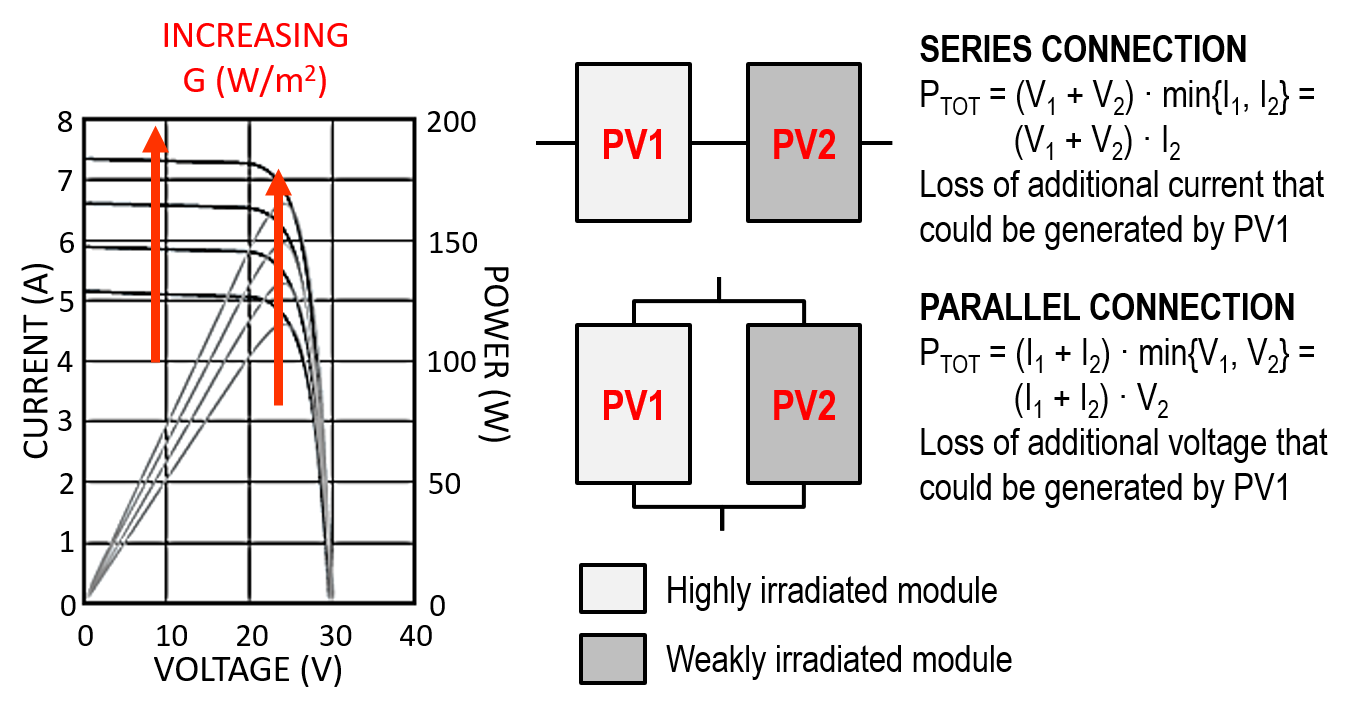
\includegraphics[width=\linewidth]{images/pv_background.png}\vspace{-0.3cm}
\caption{Typical voltage-current (I-V, black) and voltage-power (P-V, gray) curves of a PV module \cite{datasheet} (left), and impact of partial shading on the series or parallel connection of PV modules (right).
}
%\vspace{-0.5 cm}
\label{fig:moduleStructure}
\end{figure}

In any PV installation PV modules are typically connected in series or in parallel to achieve the desired voltage and current levels (right of of Figure~\ref{fig:moduleStructure}). %: the typical connection is organized as a number of parallel strings, each composed of the same number of PV modules connected in series. 
If two connected PV modules work with the same input irradiance, then their connection doubles the output power production. However, this is rarely the case, above all in urban areas where obstacles such as chimneys, surrounding buildings, trees, etc project shadows and determine a heterogeneous distribution of irradiance \cite{LI2020118795}. 
%\subsection{Impact of partial shading on PV production}\label{sec:back_pv:shading}
%In urban areas,\cite{LI202 0118795}. 
%PV installations are typically designed by assuming that the surface of interest is subject to even irradiance. This is however not accurate, as shadows projected by obstacles such as chimneys, surrounding buildings, trees, etc determine a heterogeneous distribution of irradiance, with the effect that each PV module will operate at different irradiance conditions. 

Shading is critical for PV installations, as the least irradiated PV module acts as a bottleneck on power production: the higher the variance of irradiance, the higher the power loss (right of of Figure~\ref{fig:moduleStructure}). 
When PV modules are connected in series, the least irradiated module will provide the smallest current; when PV modules are connected in parallel, the PV module with lowest voltage will determine the voltage of all connected PV modules. 
%This leads to a potentially high power dissipation, resulting in local overheating,  accelerated ageing and permanent cell damage \cite{6528850}. 



\section{Methodology}\label{sec:method}
\section{Methodology}
\label{sec:method}
evaluation of the irradiance traces for the roof all of the district

evaluation of the 75 percentile for the traces


Find all the possible position inside the available surface, sort them by the 75-th percentile, eliminate the panel with percentile lower than a threshold, find the configuration for the panels them taking into account distance between panels and height difference (description of the algorithm)

Given the best configuration try to place the same amount of panels on the used roof in a more classical way (classical algorithm description)

evaluate the roi given the panel costs the maintenance cost and the production

\hline
The goal of the paper is to find the best possible configuration for a PV panels system for a group of blocks of the city of Turin, considering the possibility to connect panel across contiguous roofs. The first step identifies the area of the blocks that could be exploited to install the PV panels. Then we proceed with the generation of the traces of G and T for the whole area with a fine time and space resolution (A). In the second step we evaluate a statistical measure to find which points of the suitable areas are the most illuminated during the year (B). The third step consist in the placement of the panel with a greedy approach and with a classical approach (C), then we evaluate the yearly production for bot the approaches (D).

\subsection{A}
Starting from a Digital Surface Model the algorithm identifies possible encumbrances an the evolution of the shadows to find the possible areas of the roof which could be used for the panel deployment. (Spiegazione di come funziona l'algoritmo che trova area_suit, forse lo avevamo fatto anche al corso di dottorato? @Lorenzo)
This step also allows us to know the inclination and the aspect of the roof that will be used in the following steps of the proceure.
The first part of the algorithm exploits high resolution maps of irradiance and temperature generated by the framework developed in [primo articolo]
Using the suitable areas indetified before the value of the irradiance over the time is evaluated by using together weather data and the shadow model. The spatial resolution of this traces is the same one of the DSM (i.e. 1 m) while the time resolution is 15 minutes. 

\subsection{B}
The following step consists in the calculation of the 75-th percentile for each point of this suitable areas, these values allows us to identify the more illuminated points to be used for the PV panel placement. 
The second part finds all the possible places where a single panel could be placed, the dimension of the panel to consider and the resolution of the search can be defined by the user. For each of this position we calculate a performance indicator as the minimum 75-th percentile of the points that intersects the panel surface, then we sort the list of those positions according to that value.
For this list of panels positions we defined different threshold values for the performance indicator to limit the number of positions to consider for the following steps.

\subsection{C}
The third part of the algorithm uses the list of panels posiiton fouund in the previous step to find an optimal panel configuration. 



\section{Results}\label{sec:results}
% Descrivere l'area utilizzata con foto di area con sovrapposta area suitable, differenza tra area dei tetti e area suitable per far notare come non sia fatto a caso. Quanta della suiatable are è stat utilizzata per il deployment. Andamento roi per i diversi valori della threshoold. Paragone classic vs greedyq3

%Fare foto con differenza di treshold da satellite,
% vedere se si riece a calcolare quanto si sovrappongono le soluzioni optimal vs classical
%Figura 2 trovare tetto con percentile che non fuoriesce

\subsection{Suitable area identification and optimization}
We tested the proposed framework on a district of  \omitted{the city of Turin} represented in Figure \ref{fig:satellite}. The satellite view of the area used for the test is overlapped with the result of step \ref{subsec:suitablearea}: the green area represents the total surface of the roofs (around $1,700,000m^2$, i.e., $1.7km^2$), while the red area represents the area that is suitable for PV installation (about $8340m^2$). It is interesting to notice that just 0.5\% of the available roof surface is considered suitable for PV installation. \attenzione{This underlines that the DSM data management strategy followed in this work allows to optimize data memorization, as only few DSM points are used to filter the suitable area, and full irradiance traces are generated only for a very limited portion of the district.} %analysis like the one proposed by our framework are extremely important to maximize the value of the investment for an EA, and that the DSM data management strategy adopted in this work allows to optimize data memorization to cover a large area.} 
 
\subsection{Optimal placement setup}
In our setup, we consider a PV-MF165EB3 module by Mitsubishi \cite{datasheet} organized in strings of 8 PV modules. The algorithm is set to allow maximum distance among panels on the same series $maxD$ of 3 meters, and a maximum height difference $maxH$ in the same series of 0.5 meters. This configuration allows to place in the same series PV modules positioned on different but almost contiguous roofs. An example of this scenario is visible in the top of Figure \ref{fig:satellizeZoom}, \attenzione{where it can be noted that the left portion of the suitable area spans across two roofs.}
\begin{figure}[!htbp]
\centering
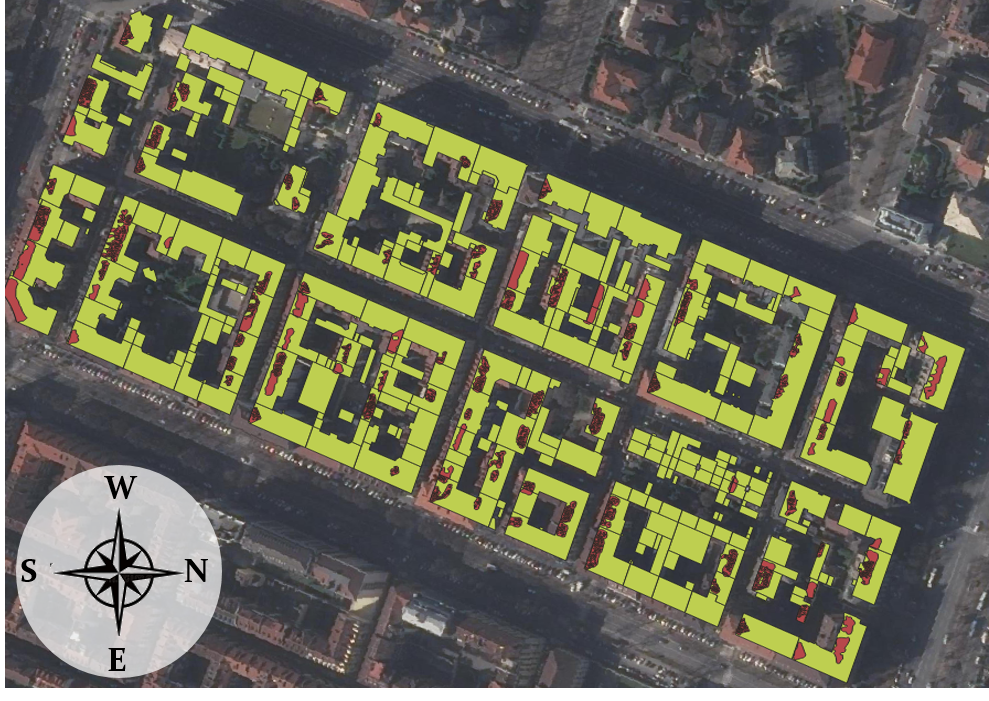
\includegraphics[width=\linewidth]{images/satellite3.png}\vspace{-0.4cm}
\caption{Satellite view of the area used for the test}
\label{fig:satellite}
\end{figure}

\subsection{Analysis of the identified PV placements}
%spiegare come si trasforma la suitable area per calcolare le tracce, tool utilizzati. menziorare il fatto che parto dal dsm identifico i tetti, per ogni tetto trovo la suitable area e trovo l'altezza e me la segno. Spiegare meglio il come si passa da dsm a tracce
To test the performance of the placement, we executed the algorithm multiple times with different values of $minTh$, i.e., the threshold of the 75-th percentile used to consider only the most promising portion of the suitable area. The results are reported in Table \ref{tab:areaused}. When increasing $minTh$, the area considered promising is reduced as a number of suitable locations are removed as featuring a 75th percentile lower than $minTh$. Thus, both the percentage of exploited area and the number of placed PV modules decrease when increasing $minTh$. 
% In Table \ref{tab:areaused} we can see how increasing $minTh$ involves a reduction of the amount of panels placed, as an effect of a reduction of the percentage of exploitation of the suitable area (as a lower portion of the roof has 75th percentile larger than $minTh$). 
An example is shown in Figure \ref{fig:satellizeZoom}: when $minTh$ is set to 100, 21\% of the available surface is considered suitable for PV placement; when $minTh$ is increased to 500, only 2\% of the area is considered suitable for PV installation, and as a result far less PV modules (colored rectangles) are installed on the same portion of roof. %\attenzione{forse avrebbe più senso far vedere cosa succede con 100 e 400? così serve a poco}
If we plot the number of PV modules installed (top of Figure \ref{fig:production}), we can observe that the decrease is not linear w.r.t. the threshold: as an example, moving from 200 to 300 the number of panels (and the area exploited) are reduced by $2/3$, as a wide percentage of locations has 75th percentile between 200 and 299. %In the following subsections we will see the effect of this behaviour on the power production and on the payback time.
% \begin{tabular}{|p{2.5cm}|p{0.8cm}|p{1.2cm}|p{1.5cm}|}
%\hline
%\textbf{75-th percentile threshold ($minTh$)} & \textbf{\# of panels} &\textbf{Installation area  ($m^2$)} &\textbf{Suitable area used (\%)} \\
\begin{table}[!tbp]
%\resizebox{\linewidth}{!}{%
\caption{Percentage of area used by PV placement over the total suitable area when varying $minTh$ }
\label{tab:areaused}
\centering
\begin{tabular}{|r|r|r|r|}
\hline
\textbf{Threshold} & \textbf{Panels} &\textbf{Installation} &\textbf{Suitable area} \\
\textbf{($minTh$)} & \textbf{(\#)} &\textbf{area ($m^2$)} &\textbf{used (\%)}\\
\hline\hline
100 & 1,792 & 1,540 & 21 \\\hline
200 & 1,536 & 1,319 & 18 \\\hline
300 & 656 & 561 & 8 \\\hline
400 & 464 & 394 &6 \\\hline
500 & 176 & 148 & 2 \\\hline
\end{tabular}%
\end{table}

\begin{figure}[!tbp]
\centering
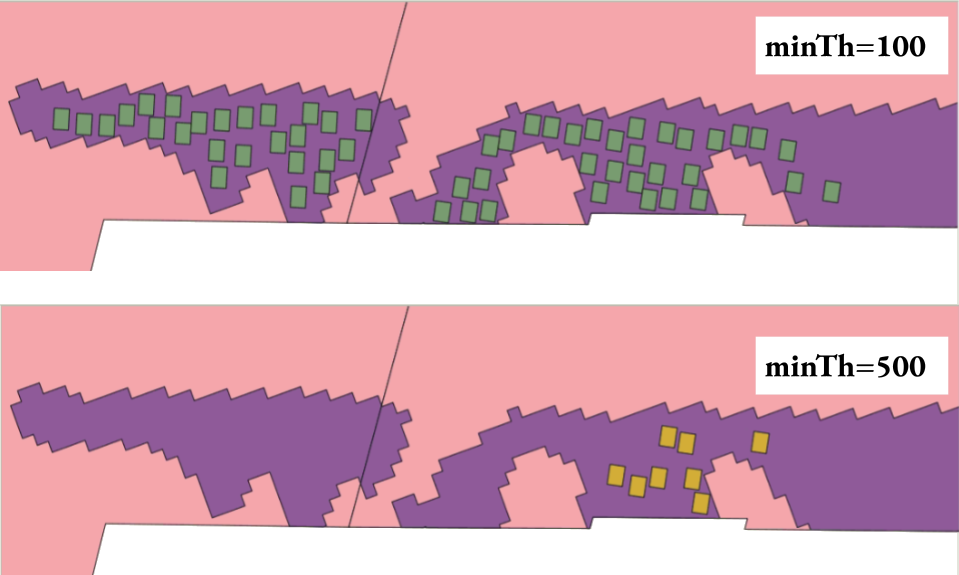
\includegraphics[width=0.9\linewidth]{images/100vs500.png}\vspace{-0.4cm}
\caption{{Result of the placement algorithm on a small portion of the district (i.e., two roofs) with threshold $minTh=100$ (top) and $minTh=500$ (bottom): the pink area represents the area of the roofs, the purple area is the suitable area, and the rectangles represent PV modules placed on locations with 75th percentile higher than $minTh$. As expected, the second placement contains less PV modules, as the minimum threshold is set to a higher value. }}
\label{fig:satellizeZoom}
\end{figure}

\subsection{Energy production performance}
To analyze the performance of the algorithm in terms of power outcome, we compared the yearly production of the identified optimal placements w.r.t. a traditional placement of the same number of PV modules. The traditional placement is built by positioning PV modules in a more standard positioning (i.e., a \virgolette{compact} rectangular placement that does not consider the 75th percentile of irradiance).
% them in the suitable area but with a more standard positioning (i.e., a \virgolette{compact} rectangular placement that does not consider the 75th percentile of irradiance), built by the algorithm proposed in \cite{soarespredicting}. Consider that the traditional placement is positioned in the suitable area and thus benefits from the preliminary analysis of irradiance and of shadow distribution, thus being a competitive placement.  
%To analyze the performance we compared the result of the energy production for the configurations obtained with our algorithm with classical configurations with the same amount of panels. The classical configurations were obtained with a custom implementation of the algorithm described in \cite{soarespredicting} that did not take into account the limitation imposed by the threshold on the irradiance. 

Table \ref{tab:production} shows that the production of the optimal PV installations is always larger than the one of the corresponding traditional placement, and as expected the production of the different configuration decreases linearly with the number of panels installed. However, it is interesting to notice that the improvement of power production is higher with higher values of $minTh$, with maximum improvement of 21\% with threshold 500 (as shown in the Table and reported in the third plot of Figure \ref{fig:production}). This behaviour can be easily explained by considering that the lower the threshold the higher the number of PV panels, and thus of potential overlap of positions of PV modules for the two placements. Vice versa, with higher thresholds the number of PV modules is reduced and the optimal placement can succesfully select only the positions less affected by shading. This reduces the impact of the bottleneck effect of partial shading on the output power production of the optimal PV placement. This analysis is confirmed by the amound of area shared by the two placements, that is higher with $minTh=100$ (36\%) and decreases with higher values of $minTh$, with a minumum of 15\% with $minTh=500$.  
% is due to the fact that having an high threshold for the 75-percentile of the irradiance allow the algorithm to use only the best positions for the panel thus reducing the impact of shading and the bottleneck effect that is normally caused by the least irradiated PV modules.%from the result summarized in the Table \ref{tab:production} and shown in plot 3 of Figure \ref{fig:production} that the optimal placement bring better result w.r.t. the classical placement when the number of panels is lower with up to a 21\% of improvement in the performance when the threshold is at 500. This behaviour is due to the fact that having an high threshold for the 75-percentile of the irradiance allow the algorithm to use only the best positions for the panel thus reducing the impact of shading and the bottleneck effect that is normally caused by the least irradiated PV modules.

% \begin{table}[!tbp]
% \centering
% %\resizebox{\linewidth}{!}{%
% %\begin{tabular}{|p{1.5cm}|p{1.5cm}|p{1.5cm}|p{1.5cm}|p{1.5cm}|}
% %\hline
% %\textbf{75-th percentile threshold} &\textbf{N of panels}&\textbf{Classic \newline configuration $P_{yearly}$(MW)}  & \textbf{Optimal \newline  configuration $P_{yearly}$(MW)} &\textbf{Improvement of optimal vs. classic} \\

% \begin{tabular}{|r|r|r|r|r|}
% \hline
% \textbf{Threshold} & \textbf{Panels} & \multicolumn{2}{c|}{\textbf{Power production (MW)}} & \textbf{Improvement}\\
% \cline{3-4}
% \textbf{($minTh$)} & \multicolumn{1}{c|}{\textbf{(\#)}} & \textbf{Optimal} & \multicolumn{1}{c|}{\textbf{Traditional}} & \multicolumn{1}{c|}{\textbf{(\%)}}\\
% \hline\hline
% 100 & 1,792 & 1,015 & 998 & 1.6\% \\\hline
% 200 & 1,536 & 905 & 874 & 3.6\% \\\hline
% 300 & 656 & 423 & 376 & 12.6\% \\\hline
% 400 & 464 & 323 & 277 & 16.9\% \\\hline
% 500 & 176 & 139 & 115 & 20.8\% \\\hline
% \end{tabular}%
% \caption{Summary of the comparison among the optimal placement with varying $minTh$ w.r.t. a traditional placement of the same number of panels \attenzione{è possibile stimare se c'è un overlap tra i due placement, i.e., quanti pannelli sono nella stessa posizione?}}
% \label{tab:production}
% \end{table}


%\resizebox{\linewidth}{!}{%
%\begin{tabular}{|p{1.5cm}|p{1.5cm}|p{1.5cm}|p{1.5cm}|p{1.5cm}|}
%\hline
%\textbf{75-th percentile threshold} &\textbf{N of panels}&\textbf{Classic \newline configuration $P_{yearly}$(MW)}  & \textbf{Optimal \newline  configuration $P_{yearly}$(MW)} &\textbf{Improvement of optimal vs. classic} \\
\begin{table}[!tbp]
\centering
\caption{Summary of the comparison among the optimal placement with varying $minTh$ w.r.t. a traditional placement of the same number of panels.}
\label{tab:production}
\begin{tabular}{|r|r|r|r|r|r|}
\hline
\textbf{Threshold} & \textbf{Panels} &\textbf{Shared} & \multicolumn{3}{c|}{\textbf{Power production (MW)}} \\
\cline{4-6}
\textbf{($minTh$)} & \multicolumn{1}{c|}{\textbf{(\#)}} & \multicolumn{1}{c|}{\textbf{area (\%)}}& \textbf{Optimal} & \multicolumn{1}{c|}{\textbf{Traditional}} & \multicolumn{1}{c|}{\textbf{(\%)}}\\
\hline\hline
100 & 1,792 &36 & 1,015 & 998 & +1.6\% \\\hline
200 & 1,536 &31 & 905 & 874 & +3.6\% \\\hline
300 & 656 &22 & 423 & 376 & +12.6\% \\\hline
400 & 464 &23 & 323 & 277 & +16.9\% \\\hline
500 & 176 &15 & 139 & 115 & +20.8\% \\\hline
\end{tabular}%
\end{table}

\begin{figure}[!tbp]
\centering
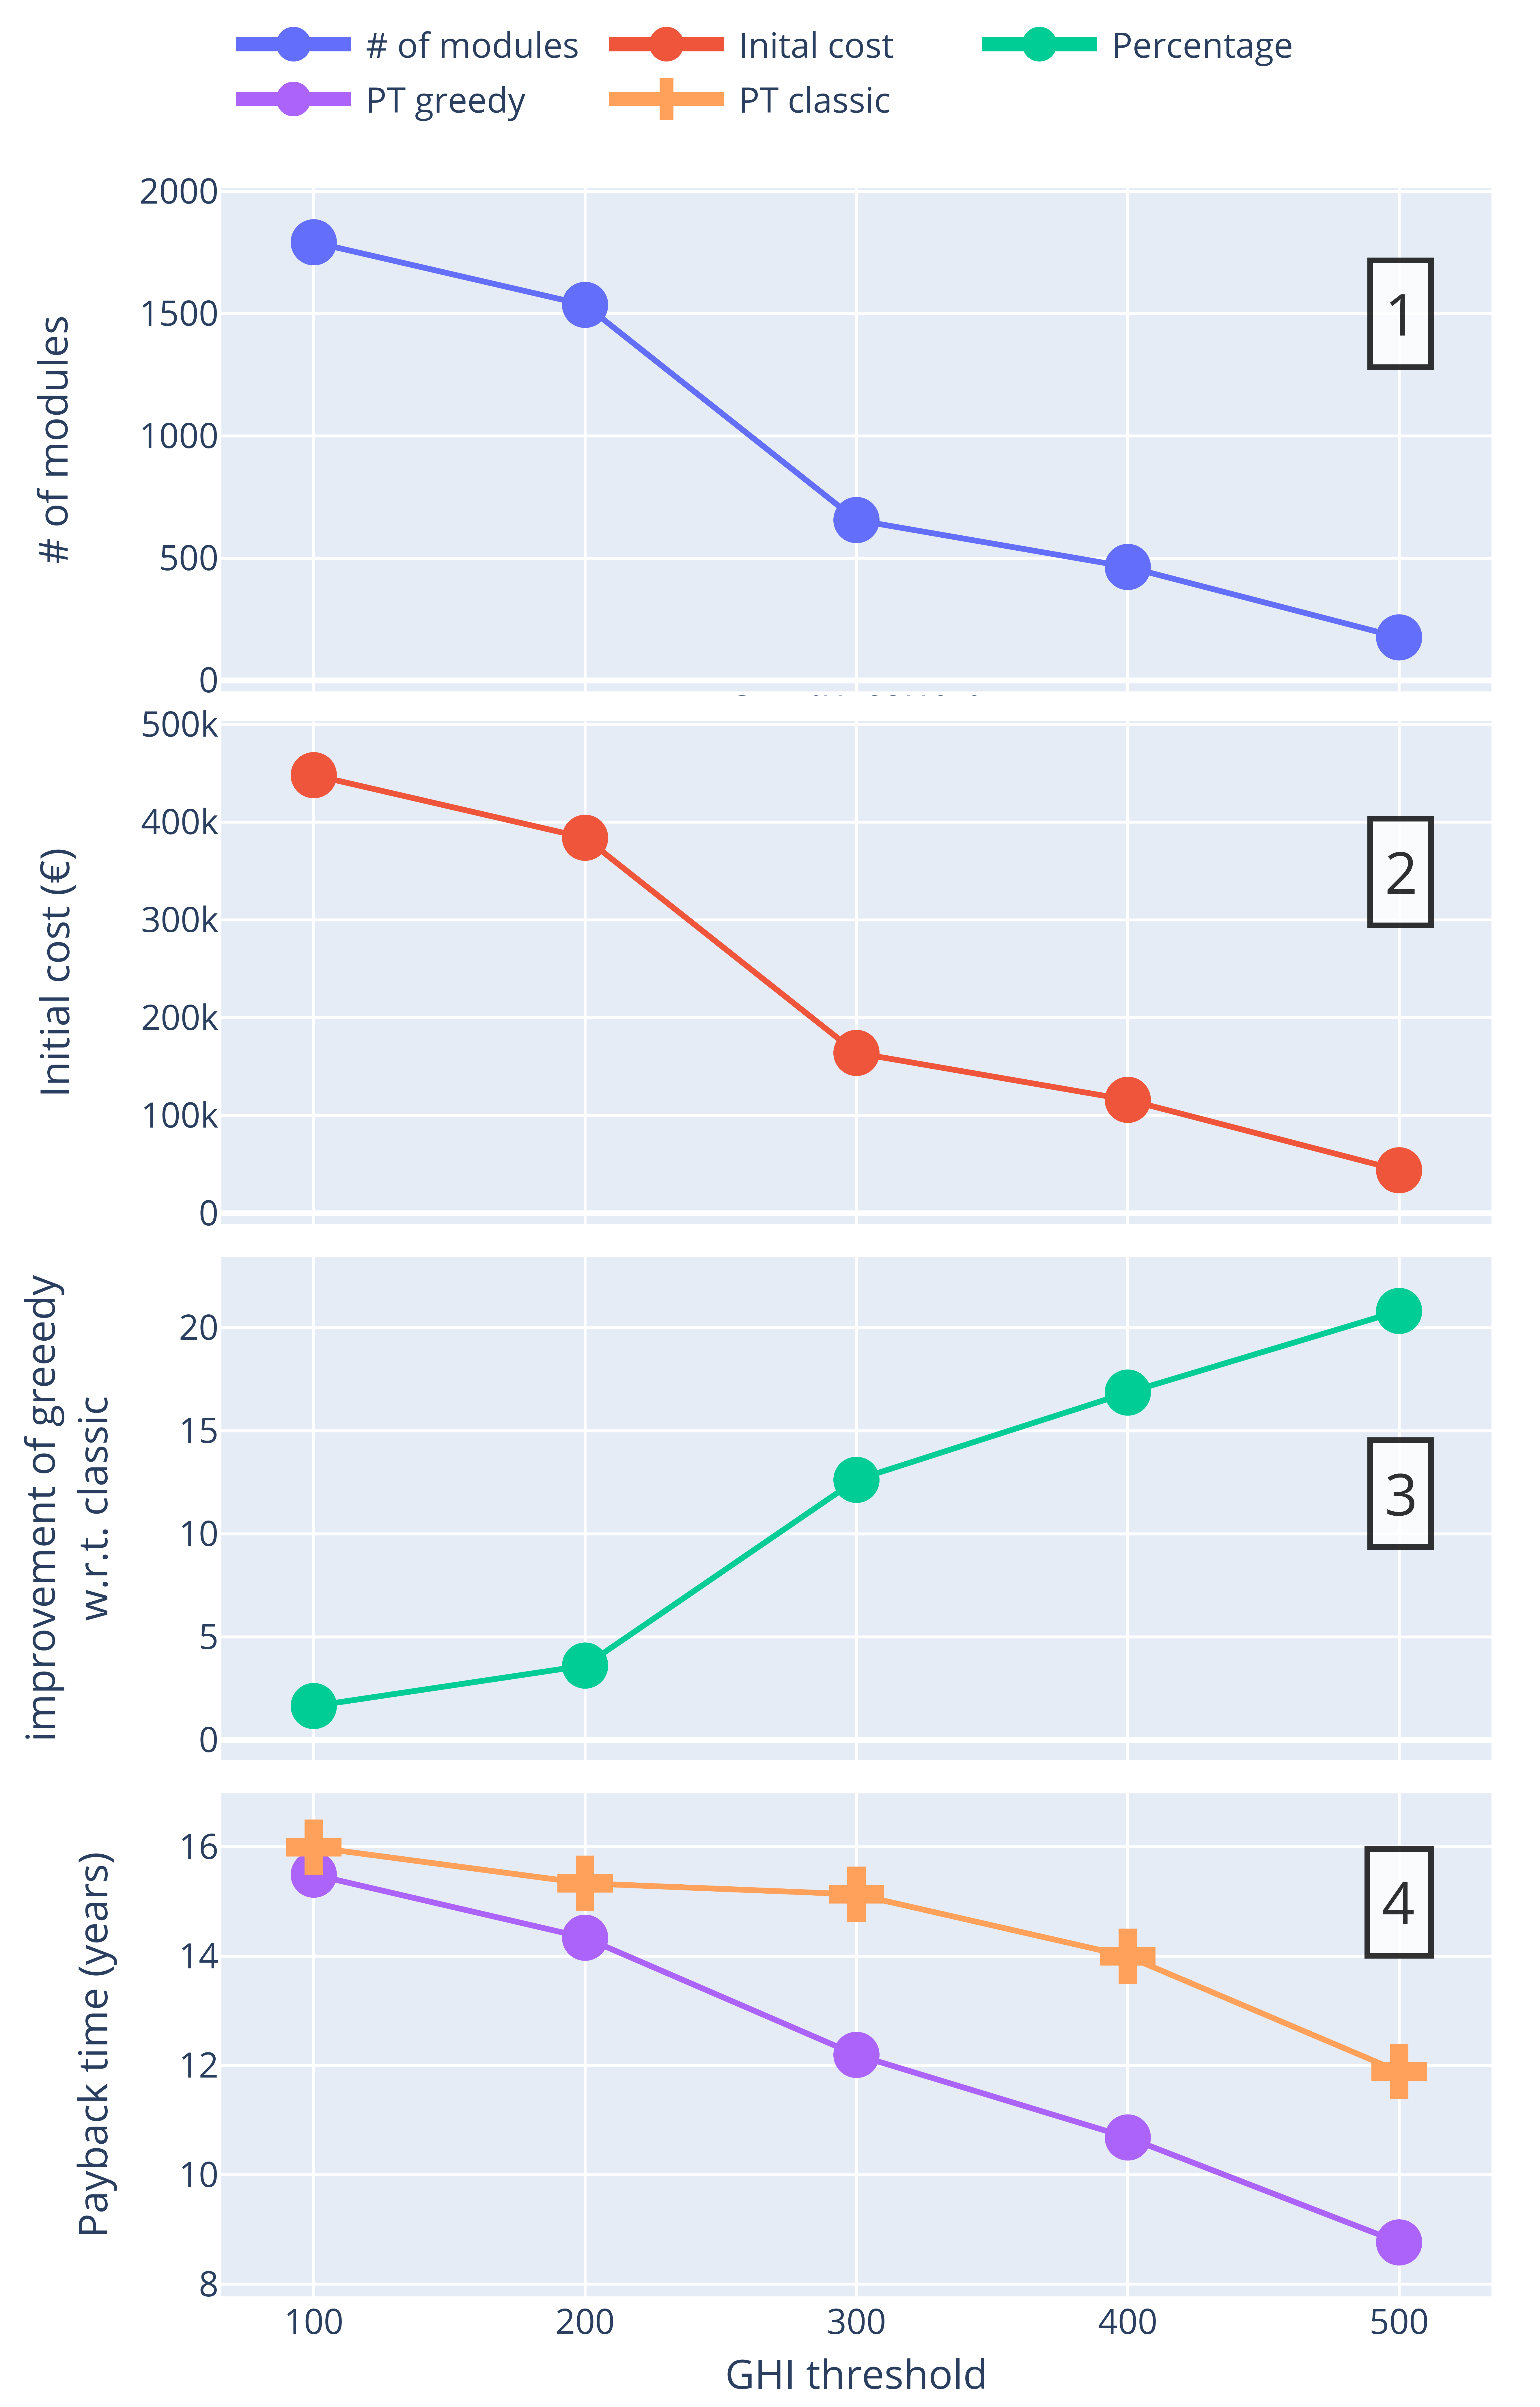
\includegraphics[width=\linewidth]{images/stacked_annotated2.png}\vspace{-0.4cm}
\caption{Behavior of the placement algorithm with different values of $minTh$: number of PV modules (1), initial installation cost (2), improvement of power production w.r.t. the traditional placement (3), payback time (4) (orange for the proposed algorithm, purple for the traditional placement).}
\label{fig:production}
\end{figure}
\subsection{Payback time}
Using the procedure explained in \ref{sec:economic} we evaluated the PT for both the classic and the optimal configuration considering also the different value of the threshold. The energy price considered is 0.22€ per kWh \cite{energy_price}, the panel cost is 250€ per panel and the maintenance cost considered is 15€ per panel per year. The plot 4 in Figure \ref{fig:production} shows how the PT decreases together with the number of panels and that the payback times of the PV installation produced by our framework are always lower than the classical ones. In particular when the threshold is at 500 the configuration produced by the framework reduces by $1/4$ the PT. However by comparing the result in \ref{tab:production} and the Figure \ref{fig:production} we can notice while increasing the amount of panels increases the production and therefore the earning this does not decrease the PT that instead increases. This underlines how this kind of analysis are useful for an EA that needs to take into account this economic analysis to plan his investment.


% correggere reference al grafico, aggiungere unita di misura all'asse y e nome asse x con descrizione, scrivere meglio didascalia figura, aggiungere numero ai grafici per citarli nel testo



\section{Conclusions}\label{sec:concl}
The paper proposed a framework to support optimal installation of PV modules in a city district, with the goal of maximizing the profit for an EA. The approach is based on an efficient management of DSM data, that generates detailed irradiance traces only for the promising portion of the district roofs ($\sim0.5\%$ of total district area). The data is then used to build an optimal placement of PV modules, that can be parametrized to exclude positions affected by shading and by a discontinuous irradiance over time. The determined placement allows to find the suitable trade-off between initial investment, power production and payback time of the installation, and proved to generate a surplus power production of up to $+20\%$ w.r.t. a traditional installation. \attenzione{Future work?}

\bibliographystyle{IEEEtran}
\bibliography{Biblio}

\end{document}
